\section{Data-driven Background Estimation}
\label{sec:compare}

In this analysis the background composition is not used to determine the amount of
expected background, which is directly fitted to the data mass spectrum, but is
needed to optimize the background modeling used in the signal extraction. As outlined
in \refS{sec:event} the main backgrounds in the \HToZg search originate
from SM $Z+\gamma$ and $Z+\text{jets}$ events, with 
small contributions from $t \bar t$ and $WZ$ events.
After the full selection the relative contributions from the different backgrounds
to the selected data are 82\%, 17\%, and 1\% for $Z+\gamma$, $Z+\text{jets}$ and
$t\bar t$, respectively.

\subsection{The two-dimensional sideband (ABCD) method}
In this section a data-driven estimation of the background composition is
performed. The data-driven estimation is based on the fact that after subtracting
the $t \bar t$ and $WZ$ contributions (the electroweak background), 
the sample is composed of two categories
of events that can be discriminated by looking at the properties of the 
photon candidate. In $Z+\gamma$ events, the photon candidate is a 
prompt photon\footnote{A prompt photon is defined experimentally as an
isolated, high $\pt$ photon.},
which gives rise to a narrow energy cluster in the electromagnetic calorimeter and
is usually isolated from hadronic activity. In contrast, photons in $Z+\text{jets}$
events are the result of the decay of a neutral meson (typically a $\pi^0$)
carrying a large fraction of the initial parton energy and giving rise to an
energy cluster in the electromagnetic calorimeter which is usually energetic,
has non-negligible leakage in the hadronic calorimeter, and is not isolated from
hadronic activity, as the other particles in the same jet deposit energy in the
calorimeters near the photon candidate. Therefore, we use photon identification
and isolation variables to discriminate on a statistical basis $Z+\gamma$ and
$Z+\text{jet}$ events in data. A comparison of an actual photon shower shape
with a similar shower caused by a $\pi^0$ in the ATLAS detector are presented
in \refF{fig:photonshowers}. This technique was developed and utilized
by ATLAS in the measurement of the Standard Model prompt photon production
cross section \cite{Aad:2010sp}. 

\begin{figure}[htbp]
   \centering 

    \begin{subfigure}[b]{0.45\textwidth}
        \centering
        \includegraphics[scale=0.5, angle=0]{./figures/nicephoton}
        \caption{}
        \label{fig:nicephoton}
    \end{subfigure}
    \quad 
    \begin{subfigure}[b]{0.45\textwidth}
        \centering
        \includegraphics[scale=0.5, angle=0]{./figures/fakephoton}
        \caption{}
        \label{fig:fakephoton}
    \end{subfigure}
    \caption{A nice photon candidate (Fig.~\ref{fig:nicephoton}) and a fake photon 
    (Fig.~\ref{fig:fakephoton}) candidate as seen by the ATLAS electromagnetic
    calorimeter. Notice that the photon in \refF{fig:nicephoton} is well isolated
    from other particle showers, while the photon in \refF{fig:fakephoton} is not.}
    \label{fig:photonshowers}
\end{figure}

In the two-dimensional plane formed by the photon transverse energy and
the photon tight identification variable, we define four regions:
\begin{itemize}
 \item Tight and isolated region (\textbf{signal region A}):\\
 isolated ($\et^{\text{iso($\Delta R < 0.4$)}} < 4 \GeV$) photon candidates 
 passing the tight selection criteria (mostly $Z+\gamma$ events). 
%
 \item Tight but not-isolated region (\textbf{control region B}):\\
 tight, non-isolated ($\et^{\text{iso($\Delta R < 0.4$)}} > 5 \GeV$) 
 photon candidates (non-isolated $Z+\text{jets}$ background).
%
 \item Not-tight and isolated region (\textbf{control region C}): \\
 candidates that have an isolated ($\et^{\text{iso($\Delta R < 0.4$)}} < 4 \GeV$)
 photon passing the not-tight selection (non-identified $Z+\text{jets}$ background). 
%
 \item Not-tight and not-isolated region (\textbf{control region D}): \\
 contains non-isolated ($\et^{\text{iso($\Delta R < 0.4$)}} > 5 \GeV$), 
 non-tight photon candidates ($Z+\text{jets}$ background).
\end{itemize}

\begin{figure}[!hbpt]
  \centering
  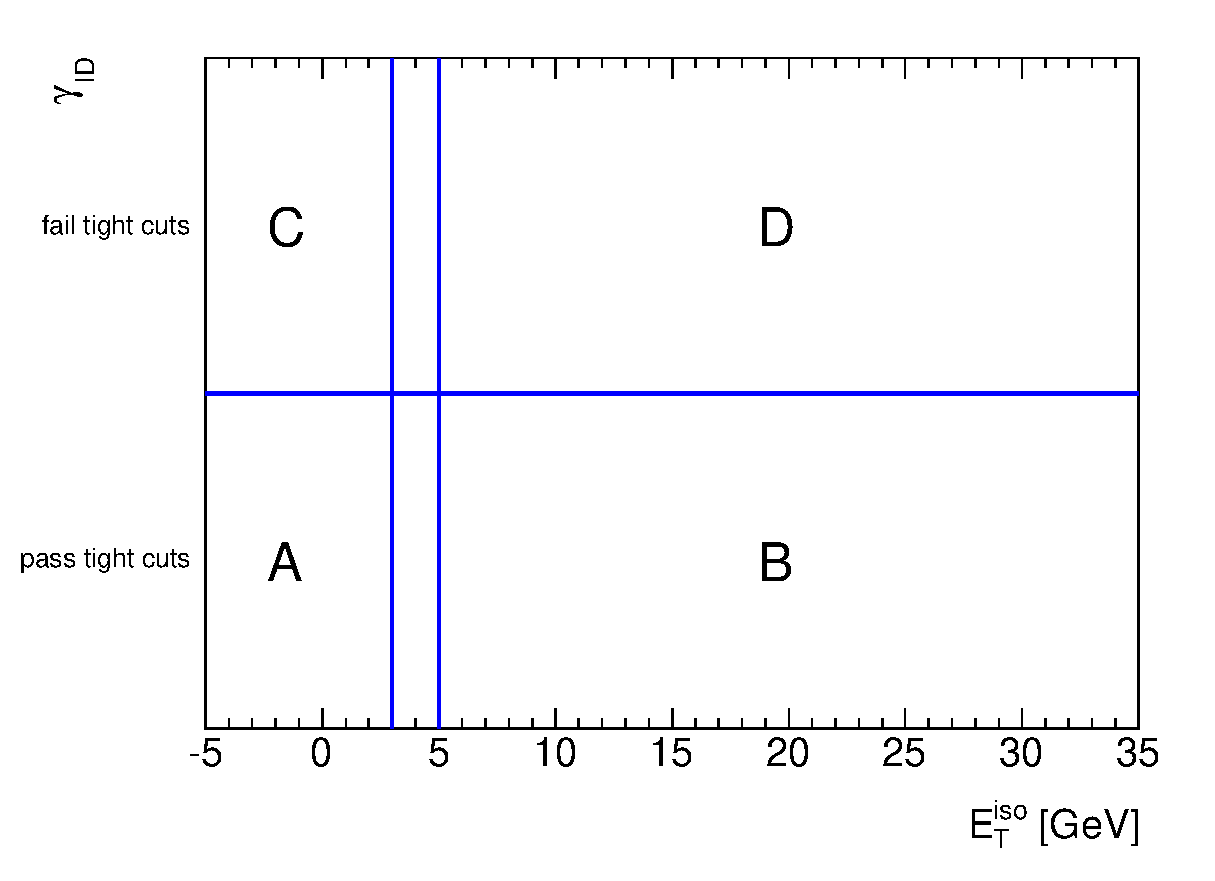
\includegraphics[scale=0.60]{figures/2dsketch.eps}
  \caption{Illustration of the two-dimensional plane, defined	
      by means of the isolation and a subset of the photon
      identification (ID) variables, from the observed yields $N_{B},
      N_{C}$ and $N_{D}$ in the three control regions, the background
    yield in the signal region were the observed total signal yield is
    $N_{A}$}
\label{fig::2dsketch}
\end{figure}

The 2D-sideband method is based on the following two assumptions: 
\begin{enumerate}
\item The signal contamination in the three background control regions (B, C, and D)
is small. This implies that all reconstructed photons falling in
one of these regions are coming from a background event. In particular, the
fraction of events coming from jet-faking events $N^{Z\text{jet}}$ can be
extracted by subtracting the contribution from electroweak backgrounds 
\New{} (estimated from Monte Carlo) from the total number of
observed events in each of these three regions: $N_A = \Nzg{A} + \Nzj{A} + \New{A}$
for the signal region and $N_K = \Nzj{K} + \New{K}$ ($K \in \{B, C, D\}$) 
for each control region.
%
\item The ratio of isolated to non-isolated background candidates from the jet-fake
in the not-tight bins $\left(\frac{\Nzj{D}}{\Nzj{C}}\right)$
is equal to the same ratio computed in the tight bins
$\left(\frac{\Nzj{B}}{\Nzj{A}}\right)$.
\end{enumerate}
These statements imply that the $Z+\text{jets}$ background in region A can
be calculated as follows:
\begin{equation}
    \Nzj{A} = (N_B - \New{B})\frac{(N_C - \New{C})}{(N_D - \New{D})}.
\end{equation}
Thus, the $Z+\gamma$ yield \Nzg{A} in region A is estimated from the number
of events in the data in the four regions as
\begin{equation}
   \Nzg{A} = (N_A - \New{A}) - (N_B - \New{B})\frac{(N_C - \New{C})}{(N_D - \New{D})}.
\end{equation}
where \New{} is estimated from electroweak background Monte Carlo simulations.

However, one must correct for the fact that the number of signal events in the
background control regions is always positive and non-zero by defining the
\emph{signal leakage fractions} $c_K = N_K^{Z\gamma\text{MC}}/N_A^{Z\gamma\text{MC}}$
that can be extracted from simulated $Z+\gamma$ samples. In addition,
there are correlations between the photon isolation variable and the
photon identification quantities that are corrected by a correlation 
coefficient
\begin{equation} 
    R^{Z\text{jetsMC}} = \frac{\Nzjmc{A} \Nzjmc{D}}{\Nzjmc{B} \Nzjmc{C}}
\end{equation}
obtained from high statistics $Z+\text{jets}$ simulated events, after removing
- using the truth information - the contributions from $Z+\gamma$ processes.
The final result for the signal yield is then
\begin{equation}
   \Nzg{A} = (N_A - \New{A}) - (N_B - \New{B} - c_B\Nzg{A})\frac{(N_C - \New{C} - c_C\Nzg{A})}{(N_D - \New{D} - c_D\Nzg{A})}\,R^{Z\text{jetsMC}}.
\label{eq:2destB}
\end{equation}
This is a second-order polynomial equation in $N_A^{Z\gamma}$ that only has
one physical solution, i.e. a positive solution. Finally, the $Z+\text{jets}$
background is obtained as
\begin{equation}
\Nzj{A} = N_A - \New{A} - \Nzg{A}.
\label{eq:2destA}
\end{equation}

\subsection{Data-Monte Carlo comparisons}
Following the discussion in the previous section the $Z$+jets background to
$Z\gamma$ processes are estimated using Equation~\ref{eq:2destA} and \ref{eq:2destB}.
In the following we define the purity ($P$) of $Z\gamma$ candidate samples as
\[
    P = \frac{N_A - \Nzj{A} - \New{A}}{N_A}.
\]
A summary of the different measured backgrounds as well as the purity of $Z\gamma$
events in data are calculated and summarized in \refT{tab:zgbgsummary}.
After the full selection the relative contributions from the different backgrounds
to the selected data are 82\%, 17\%, and 1\% for $Z+\gamma$, $Z+\text{jets}$ and
$t\bar t$, respectively.
In addition, a comparison between data and the simulation after scaling each 
MC background contribution to the number of events estimated in data is shown in 
\refF{fig:zgamma_mass_linear} and \ref{fig:Dm_mass_linear}. 
A good agreement between data and simulation is observed.

\begin{table}[!htbp]
\centering
\caption{
 Estimations of $Z$+jets and electroweak background events after all $H\rightarrow Z \gamma$ selection cuts in electron and muon categories for the 2012 and 2011 datasets, which have luminosities around 20.7 fb$^{-1}$ and 4.6 fb$^{-1}$, respectively. Errors in MC $t\bar{t}$, $WZ$ and extracted Data-Driven $Z\gamma$ events are only statistical.}
  \label{tab:zgbgsummary}
\begin{tabular}{ccccccc}
       \hline
%%      \textbf{background source } & $pp \rightarrow e^{+}e^{-}\gamma$  & $pp \rightarrow \mu^{+}\mu^{-}\gamma$ \\
       \textbf{background source } & $Z(e^{+}e^{-})\gamma$  & $ Z( \mu^{+}\mu^{-})\gamma$ \\
       \hline
 	  &   {\bf 8TeV} &  \\
       \hline
	   
      total observed events & 13898    &  16658 \\
       \hline
        $Z$+$jets$             & $ 2137.58 \pm 116.94 \pm 541.45  $ &  $ 2561.69 \pm 109.23  \pm 474.94 $  \\
       $t\bar t$            &  $ 63.08 \pm 2.65 $&  $ 78.58 \pm 3.08 $ \\
 	$WZ $   	     &  $ 9.55 \pm 0.66 $ &  $ 6.97 \pm 0.52 $    \\
       \hline
   extracted $Z\gamma$ events  & $ 11687.79 \pm 166.07  $ &   $ 14010.76 \pm 169.11 $  \\
       \hline
 	Purity   		&  $ 0.841 \pm 0.014 \pm 0.039 $             &  $ 0.841 \pm  0.012 \pm 0.028$    \\
       \hline	 
       \hline
 	  &   {\bf 7TeV} &  \\
       \hline

      total observed events & 1960    &  2665 \\
       \hline
        $Z$+$jets$             & $ 318.20 \pm 45.84 \pm 34.24  $ &  $ 343.25 \pm 39.88  \pm 21.04 $  \\
       $t\bar t$            &  $ 7.45 \pm 1.17 $&  $ 8.31 \pm 1.23 $ \\
        $WZ $                &  $ 5.63 \pm 0.19 $ &  $ 5.38 \pm 0.18 $    \\
       \hline
   extracted $Z\gamma$ events  & $ 1628.72 \pm 63.74  $ &   $ 2308.06 \pm 65.25 $  \\
       \hline
        Purity                  &  $ 0.831 \pm 0.037 \pm 0.017 $             &  $ 0.866 \pm  0.030 \pm 0.015$    \\
   \hline
   \hline
      

\end{tabular}
\end{table}

\begin{figure}[!htbp]
  \begin{center}
    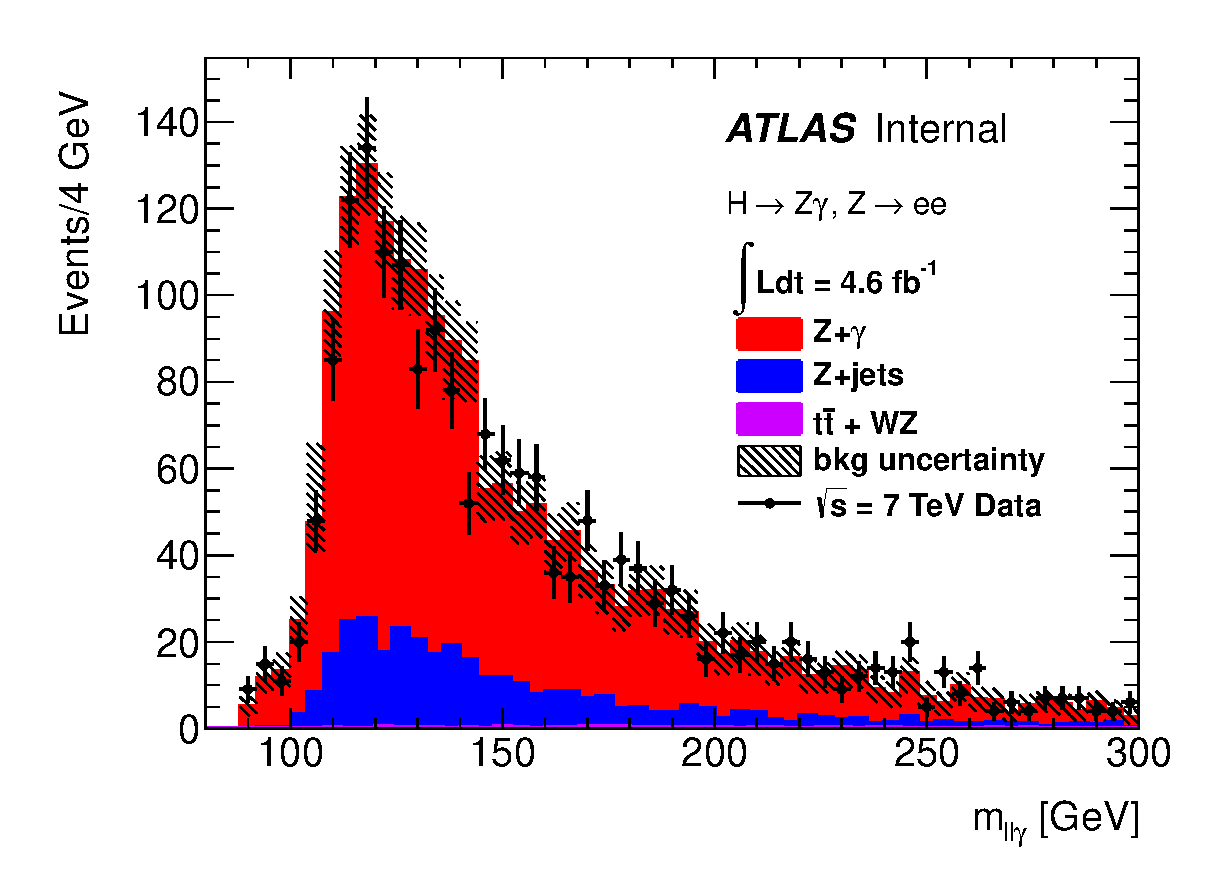
\includegraphics[width=0.49\columnwidth]{figures/bkg_decomposition_2011_e_Mllg_Z_PV_corr_linscale}
    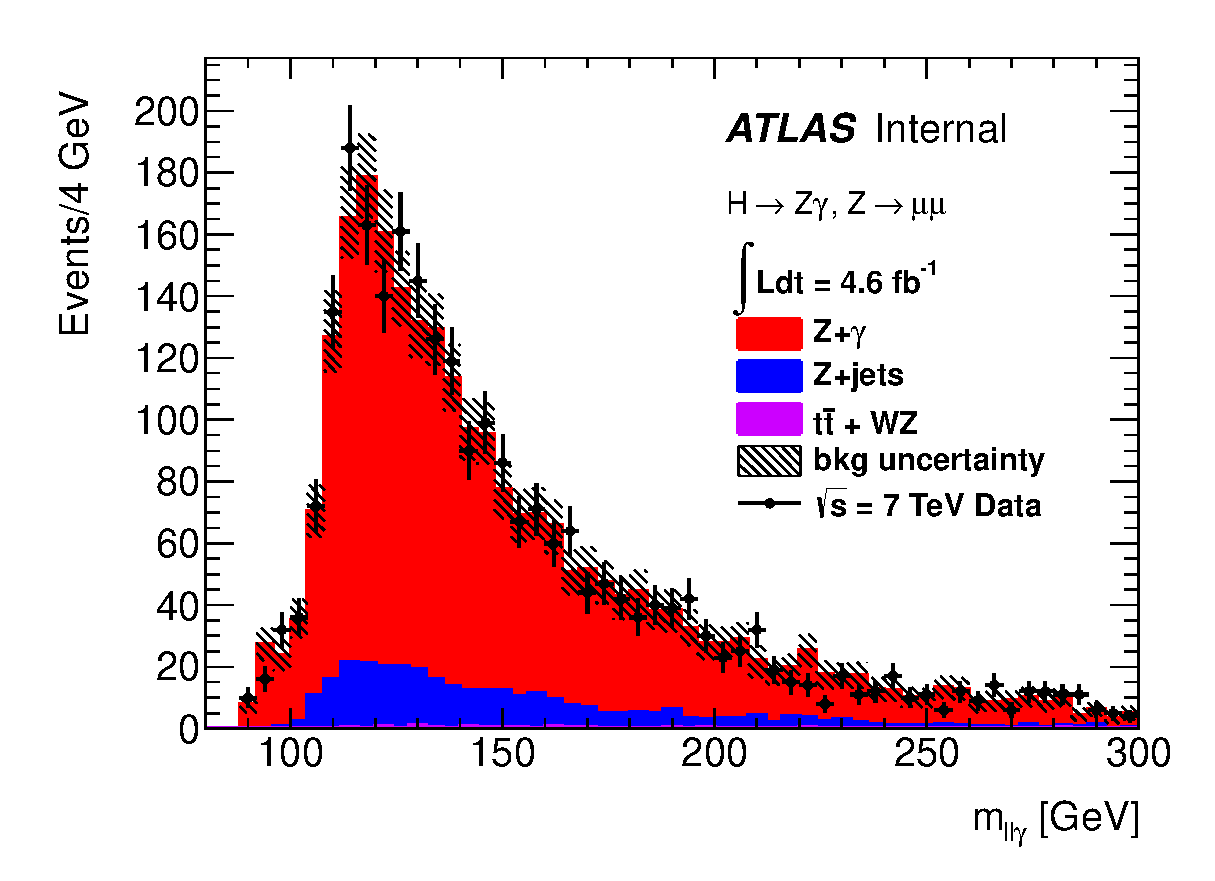
\includegraphics[width=0.49\columnwidth]{figures/bkg_decomposition_2011_mu_Mllg_Z_PV_corr_linscale}
    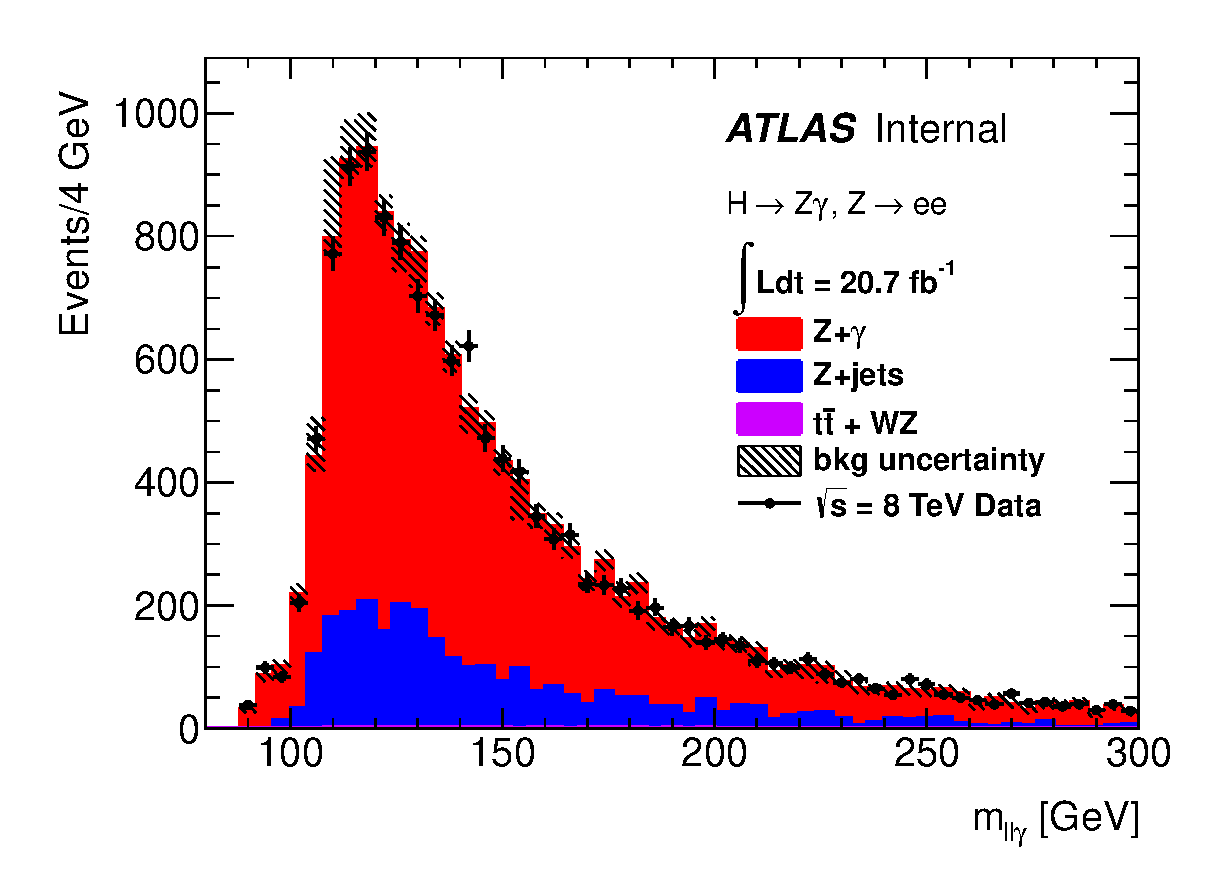
\includegraphics[width=0.49\columnwidth]{figures/bkg_decomposition_2012_e_Mllg_Z_PV_corr_linscale}
    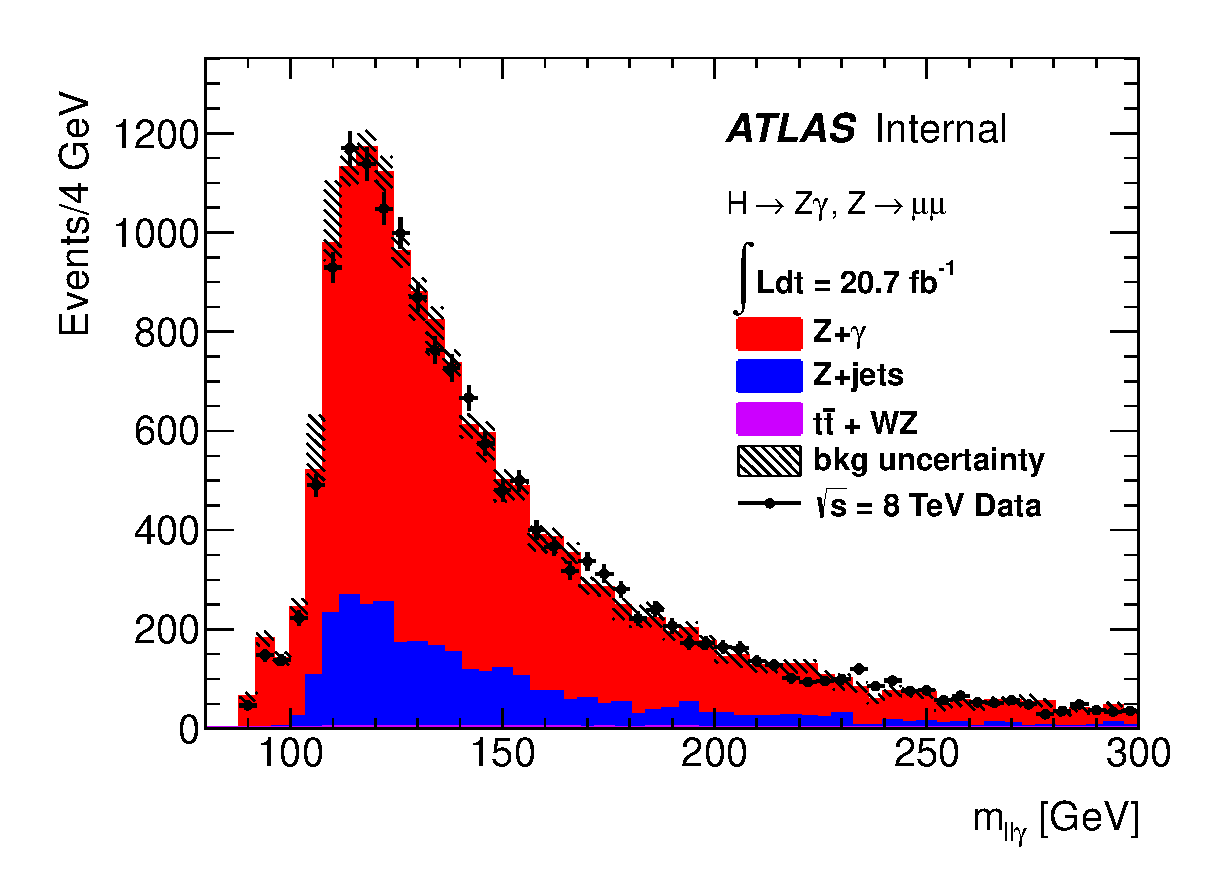
\includegraphics[width=0.49\columnwidth]{figures/bkg_decomposition_2012_mu_Mllg_Z_PV_corr_linscale}
    \caption{Three-body invariant mass $(m_{\ell\ell\gamma})$ distribution 
      of selected events in data (dots) and from the various
      background sources (histograms, from the simulation) normalized 
      to the yields determined as described in the text, 
      for $Z\to ee$ (left) and $Z\to\mu\mu$ (right) channels.
      The small peak near $m_Z$ is from residual FSR $Z$+$\gamma$ contamination.
      The background uncertainty includes statistical uncertainties and 
      systematic uncertainties from the inputs taken from the simulation, as detailed in the text.
    }
    \label{fig:zgamma_mass_linear}
  \end{center}
\end{figure}

\begin{figure}[!htbp]
  \begin{center}
    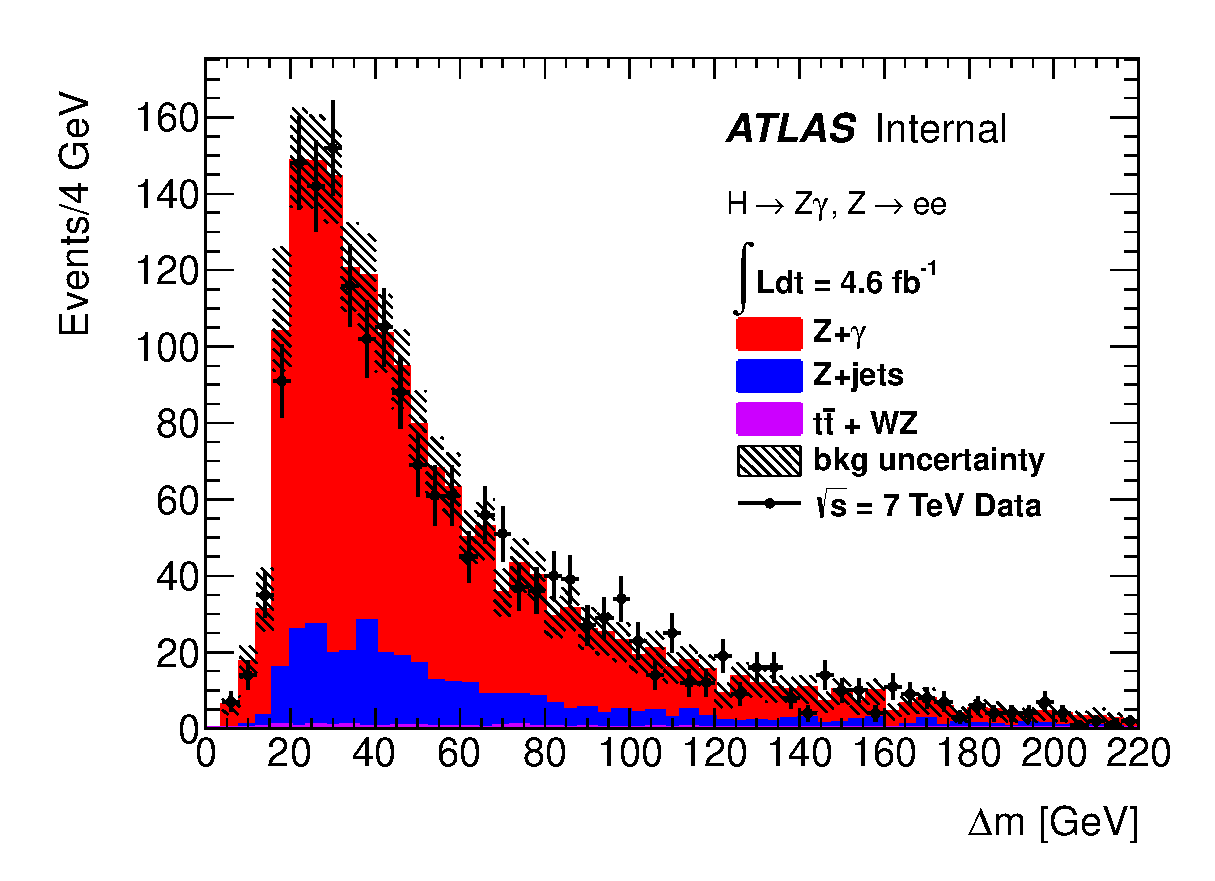
\includegraphics[width=0.49\columnwidth]{figures/bkg_decomposition_2011_e_dMllg_Z_PV_corr_linscale}
    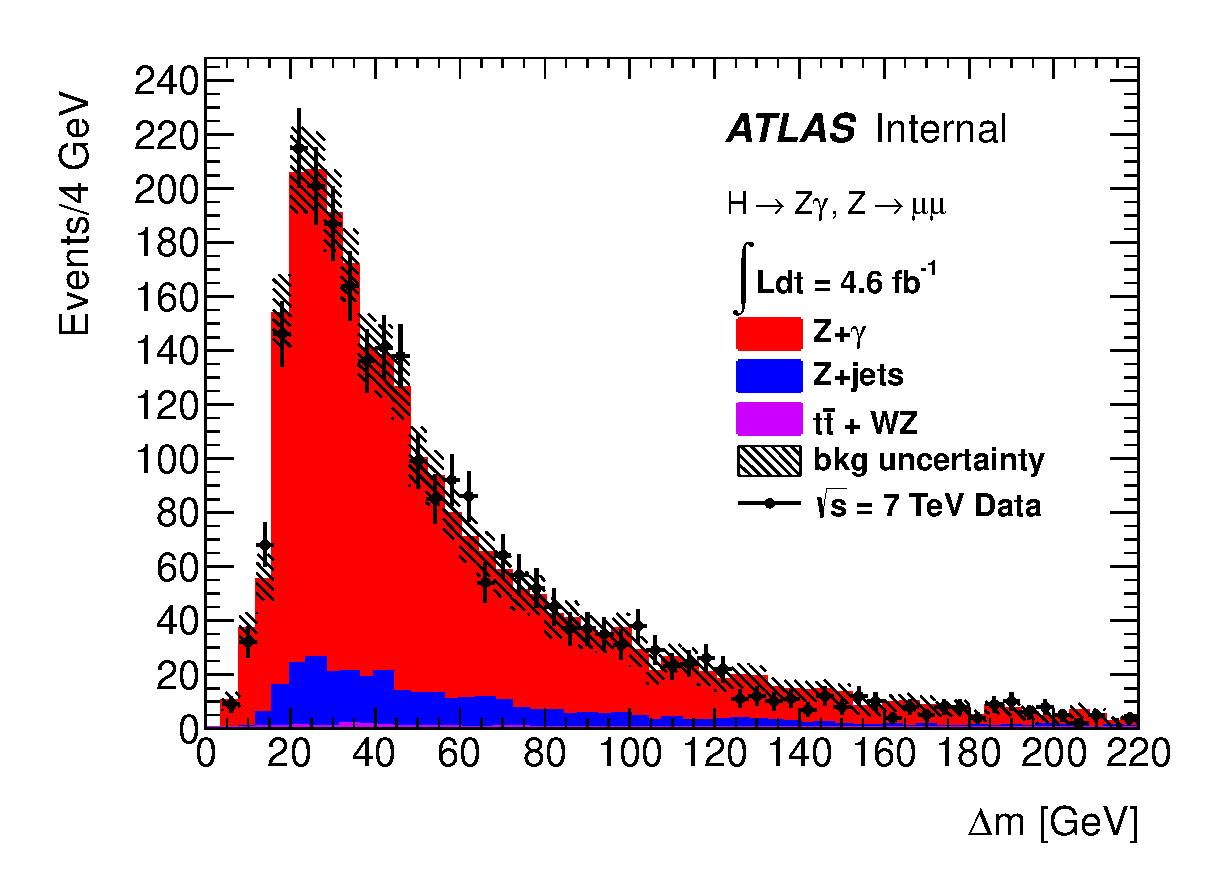
\includegraphics[width=0.49\columnwidth]{figures/bkg_decomposition_2011_mu_dMllg_Z_PV_corr_linscale}
    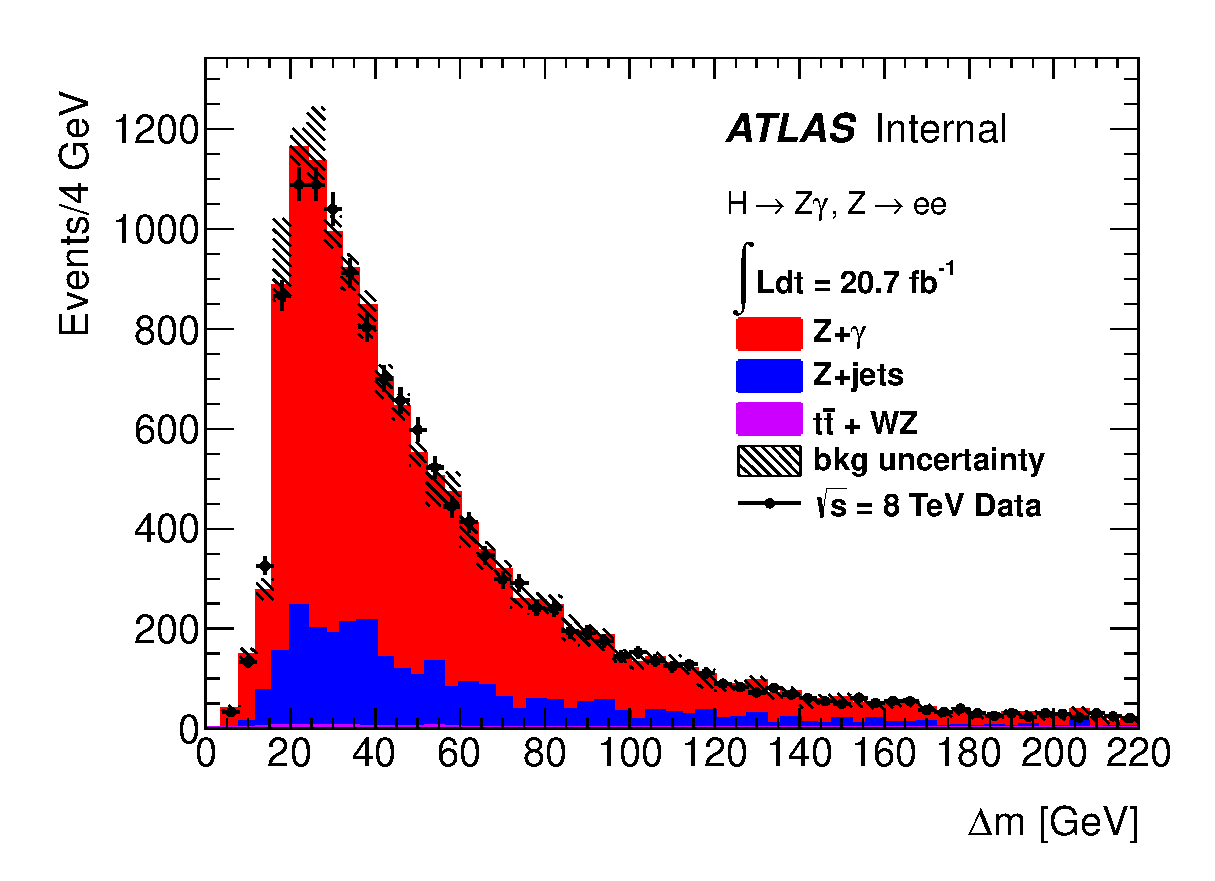
\includegraphics[width=0.49\columnwidth]{figures/bkg_decomposition_2012_e_dMllg_Z_PV_corr_linscale}
    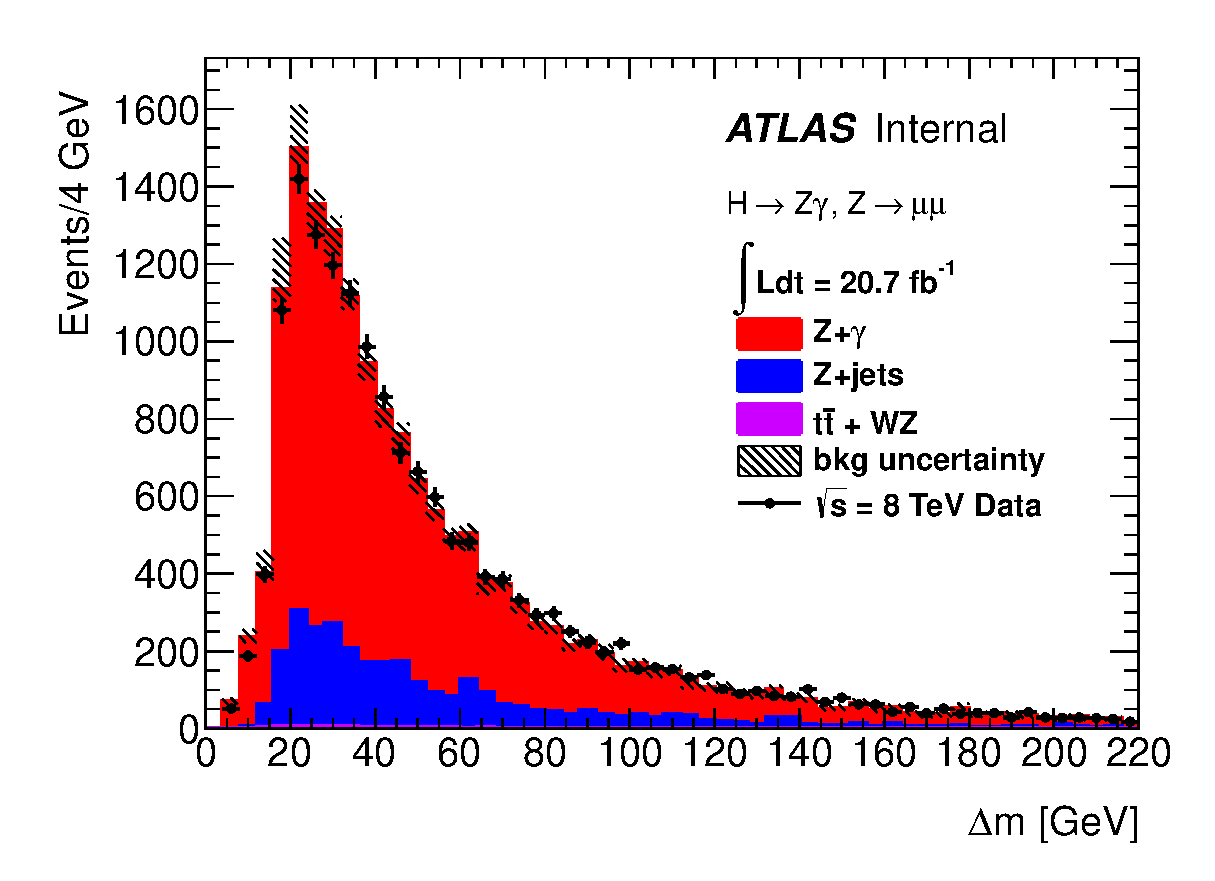
\includegraphics[width=0.49\columnwidth]{figures/bkg_decomposition_2012_mu_dMllg_Z_PV_corr_linscale}
    \caption{Distribution of the difference $\Delta m$ 
      between the final state three-body invariant mass
      $m_{\ell\ell\gamma}$ and the di-lepton invariant mass
      $m_{\ell\ell}$ for selected events in data (dots) and from
      the various background sources (histograms) normalized to the yields determined 
      as described in the text, for $Z\to ee$ (left) and $Z\to\mu\mu$ (right) channels.
      The background uncertainty includes statistical uncertainties and systematic
      uncertainties from the inputs taken from the simulation.
    }
    \label{fig:Dm_mass_linear}
  \end{center}
\end{figure}
